\chapter{Generalization, Leakage, and Evaluation Discipline}
\label{ch:evaluation-discipline}

Once a task has been framed and its success criteria have been stated, a harder question remains: when does the evidence deserve trust? Strong numbers can reflect real learning, but they can also come from leakage, weak baselines, unstable splits, or a test set that quietly became part of development.

This chapter turns evaluation discipline into procedure. It defines what should count as new evidence, how train, validation, and test roles must remain separate, and which simple checks keep a promising result honest. By the end of the chapter, the reader should be able to write a minimal evaluation plan that makes a model claim credible on genuinely new data.

\begin{learninggoals}
\item Explain why a strong-looking score is not credible without a protected evaluation workflow.
\item Distinguish training, validation, test, and external evidence roles.
\item Identify leakage, duplicate cases, weak baselines, and repeated test-set tuning.
\item Use sanity checks and simple baselines as evidence controls rather than decorations.
\item Write a minimal evaluation plan that protects a model claim on new data.
\end{learninggoals}

\begin{problemsolvinglens}
Protect the claim by keeping development, external evidence, and baseline comparison separate. A strong-looking score is not enough if the workflow that produced it made the result too easy to win.
\end{problemsolvinglens}

\begin{thinkingtool}
\textbf{Claim protection.} Before trusting a win, ask what part of the pipeline could have let future information, duplicate cases, excessive tuning, or a weak baseline make the score look better than it really is.
\end{thinkingtool}

\section{Opening Dilemma: The Validation Score Looks Great. Can We Trust It?}

Keep the same course-support setting in view from the first two chapters. Suppose a support team trains several early-warning models on historical course data and one of them produces excellent validation recall and a strong final test score. Before celebrating, the team still has to ask harder questions. Were the preprocessing steps learned only from the training data? Was the test set kept external until the end? Did the model beat a serious baseline or only an unrealistically weak comparison? Would the result still look strong next semester? Each later section of the chapter turns one of those questions into a procedural safeguard.

Those questions are not paperwork added after the model. They are what make the number mean anything.

\section{Can the Result Survive New Data? Generalization and Overfitting}

The training loss tells us how well the model matches data it has already seen. The next judgment question is whether the result survives new examples.

\begin{definition}[Generalization]
Generalization is the ability of a model to maintain good performance on unseen examples drawn from the same underlying problem as the training data.
\end{definition}

Two classic failure modes define the landscape. \emph{Underfitting} means the model is too simple, too restricted, or too poorly trained to capture even the main patterns in the training data. \emph{Overfitting} means the model matches the training data too closely, including noise or accidental details that do not hold for new data.

One way to see this is through the \emph{generalization gap}, the difference between training performance and performance on held-out data. A small gap does not guarantee excellence, but a large gap is a warning sign that the model has learned something too specific to the observed sample.

Model capacity, meaning how complex a pattern the model can represent, plays a central role here. A more flexible model can represent more complicated functions. That flexibility is useful when the data contains real structure, but dangerous when the data is limited or noisy. Overfitting is not evidence of intelligence. It is evidence that the experimental setup allowed memorization or unstable pattern matching to masquerade as learning.

If generalization is the real target, then evaluation cannot be improvised after training. It has to be built into the experimental workflow from the start.

\begin{figure}[t]
\centering
\definecolor{c3fitBlue}{RGB}{56,103,170}
\definecolor{c3fitRed}{RGB}{180,40,40}
\resizebox{\linewidth}{!}{%
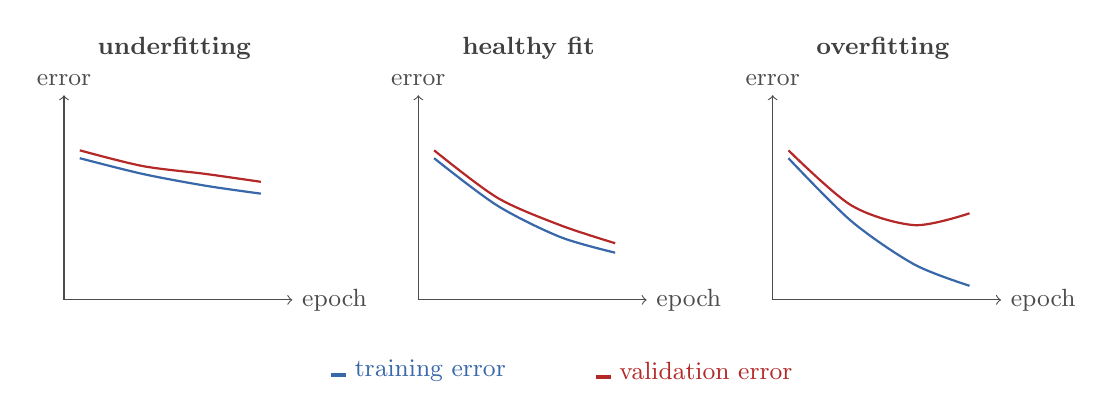
\begin{tikzpicture}[font=\small, x=1cm, y=1cm]
%% Panel 1: underfitting
\begin{scope}[xshift=0cm]
  \node[font=\small\bfseries, black!75] at (1.4,3.2) {underfitting};
  \draw[->,black!70] (0,0) -- (2.9,0) node[right] {epoch};
  \draw[->,black!70] (0,0) -- (0,2.6) node[above] {error};
  \draw[thick,c3fitBlue]  plot[smooth] coordinates {(0.2,1.8)(1.0,1.6)(1.8,1.45)(2.5,1.35)};
  \draw[thick,c3fitRed]   plot[smooth] coordinates {(0.2,1.9)(1.0,1.7)(1.8,1.60)(2.5,1.50)};
\end{scope}
%% Panel 2: healthy fit
\begin{scope}[xshift=4.5cm]
  \node[font=\small\bfseries, black!75] at (1.4,3.2) {healthy fit};
  \draw[->,black!70] (0,0) -- (2.9,0) node[right] {epoch};
  \draw[->,black!70] (0,0) -- (0,2.6) node[above] {error};
  \draw[thick,c3fitBlue]  plot[smooth] coordinates {(0.2,1.8)(1.0,1.2)(1.8,0.80)(2.5,0.60)};
  \draw[thick,c3fitRed]   plot[smooth] coordinates {(0.2,1.9)(1.0,1.3)(1.8,0.95)(2.5,0.72)};
\end{scope}
%% Panel 3: overfitting
\begin{scope}[xshift=9.0cm]
  \node[font=\small\bfseries, black!75] at (1.4,3.2) {overfitting};
  \draw[->,black!70] (0,0) -- (2.9,0) node[right] {epoch};
  \draw[->,black!70] (0,0) -- (0,2.6) node[above] {error};
  \draw[thick,c3fitBlue]  plot[smooth] coordinates {(0.2,1.8)(1.0,1.0)(1.8,0.45)(2.5,0.18)};
  \draw[thick,c3fitRed]   plot[smooth] coordinates {(0.2,1.9)(1.0,1.2)(1.8,0.95)(2.5,1.10)};
\end{scope}
%% Shared legend centered below all three panels
\node[c3fitBlue,  font=\small] at (4.5,-0.9) {\rule{0.6em}{1.5pt}\ training error};
\node[c3fitRed,   font=\small] at (8.0,-0.9) {\rule{0.6em}{1.5pt}\ validation error};
\end{tikzpicture}%
}
\caption{The same training loop can fail in three different ways. Underfitting keeps both errors high. Healthy fitting lowers both while keeping them close. Overfitting continues improving training error while validation error turns upward.}
\label{fig:underfit-healthy-overfit}
\end{figure}

\begin{evidencebox}
Zech et al.\ studied pneumonia detection from chest radiographs across multiple hospital systems and found that generalization changed substantially across institutions; they also analyzed how hospital-specific cues could act as confounders \citep{zech2018}. That is the chapter's lesson in real form: success on familiar held-out data is not the same as robust generalization after deployment.
\end{evidencebox}

\section{Protected Evaluation Workflow}

The next question is procedural rather than mathematical: how do we protect evaluation from development? The answer is the disciplined split between training, validation, and test data. This is the chapter's workflow spine, because every later safeguard depends on these roles staying distinct. The \emph{training set} is used to fit parameters. The \emph{validation set} is used to choose tuning settings, model structures, thresholds, or stopping points. The \emph{test set} is reserved for the final report after the important decisions are already made.

\begin{practicalnote}
The workflow is simple enough to say plainly: split first, fit preprocessing on train only, train candidate models on train, choose among them on validation, and touch the test set once at the end.
\end{practicalnote}

Students often understand those definitions and still run the workflow incorrectly. The key is not only what the sets are called. The key is the order in which they are used. The names matter less than the boundary: once information crosses from held-out evidence back into development, the claim is weaker even if the code still runs cleanly.

A protected test set matters not just procedurally but statistically. When a bounded metric is averaged over independent held-out examples, its empirical value concentrates around the true expected performance.

\begin{theorem}[Hoeffding Bound for Held-Out Evaluation {\citep{hoeffding1963}}]
Let $Z_1,\ldots,Z_n$ be independent random variables with $0 \le Z_i \le 1$, and let
\[
\bar{Z}=\frac{1}{n}\sum_{i=1}^n Z_i.
\]
Then for any $\varepsilon > 0$,
\[
P\!\left(\left|\bar{Z}-\mathbb{E}[\bar{Z}]\right|\ge \varepsilon\right)\le 2e^{-2n\varepsilon^2}.
\]
\end{theorem}

The practical point is not that a held-out score becomes infallible, but that an untouched test set gives a statistically interpretable estimate of performance. Repeated reuse of that same test set weakens exactly that interpretation.

If the held-out metric is an average of bounded per-example quantities, such as accuracy indicators or a loss rescaled into $[0,1]$, this inequality explains why larger protected test sets produce more stable evidence and why repeated peeking at the same hold-out set is so damaging.

\begin{mathlens}
For a rough scale check, plug in \(\varepsilon=0.10\). With \(n=100\) held-out examples, Hoeffding gives
\[
P(|\bar Z-\mathbb{E}\bar Z|\ge 0.10)\le 2e^{-2}=0.27.
\]
With \(n=1000\), the same deviation bound becomes \(2e^{-20}\), essentially zero for practical purposes. This does not mean the estimate is unbiased under distribution shift, duplicate examples, leakage, or test-set reuse. It only says that, under the stated independence and boundedness assumptions, larger untouched samples make random sampling noise smaller.
\end{mathlens}

Here \emph{preprocessing} means data transformations such as scaling, normalization, or feature extraction that are learned from the training data and then applied unchanged to validation and test data.

\begin{figure}[t]
\centering
\definecolor{c3wfRaw}{RGB}{235,242,253}
\definecolor{c3wfRawLine}{RGB}{56,103,170}
\definecolor{c3wfPrep}{RGB}{210,238,220}
\definecolor{c3wfPrepLine}{RGB}{26,112,64}
\definecolor{c3wfTrain}{RGB}{220,233,251}
\definecolor{c3wfTrainLine}{RGB}{56,103,170}
\definecolor{c3wfTune}{RGB}{254,242,214}
\definecolor{c3wfTuneLine}{RGB}{184,92,16}
\definecolor{c3wfTest}{RGB}{237,224,250}
\definecolor{c3wfTestLine}{RGB}{100,50,160}
\resizebox{\linewidth}{!}{%
\begin{tikzpicture}[x=1cm, y=1cm, font=\small,
  raw/.style ={draw=c3wfRawLine,  fill=c3wfRaw,  rounded corners, align=center,
               minimum height=0.9cm, minimum width=2.1cm,
               font=\small\bfseries, text=c3wfRawLine},
  pre/.style ={draw=c3wfPrepLine, fill=c3wfPrep, rounded corners, align=center,
               minimum height=0.9cm, minimum width=2.7cm,
               font=\small\bfseries, text=c3wfPrepLine},
  trn/.style ={draw=c3wfTrainLine,fill=c3wfTrain,rounded corners, align=center,
               minimum height=0.9cm, minimum width=2.3cm,
               font=\small\bfseries, text=c3wfTrainLine},
  tun/.style ={draw=c3wfTuneLine, fill=c3wfTune, rounded corners, align=center,
               minimum height=0.9cm, minimum width=2.1cm,
               font=\small\bfseries, text=c3wfTuneLine},
  tst/.style ={draw=c3wfTestLine, fill=c3wfTest, rounded corners, align=center,
               minimum height=0.9cm, minimum width=2.1cm,
               font=\small\bfseries, text=c3wfTestLine},
  arrow/.style={-Latex, thick, black!55}
]
%% ── Top row ──────────────────────────────────────────────────────────
\node[raw] (raw)   at (1.1,  3.2) {Raw data};
\node[raw] (split) at (3.8,  3.2) {Split first};
\node[pre] (prep)  at (7.2,  3.2) {Fit preprocessing\\on train only};
%% ── Bottom row ───────────────────────────────────────────────────────
\node[trn] (train) at (3.8,  0.9) {Train candidate\\models};
\node[tun] (tune)  at (7.2,  0.9) {Tune on\\validation};
\node[tst] (test)  at (10.3, 0.9) {Report once\\on test};
%% ── Arrows ───────────────────────────────────────────────────────────
\draw[arrow] (raw)   -- (split);
\draw[arrow] (split) -- (prep);
\draw[arrow] (split) -- (train);
\draw[arrow] (prep)  -- (tune);
\draw[arrow] (train) -- (tune);
\draw[arrow] (tune)  -- (test);
%% ── Annotation: sits to the right of the prep→tune arrow ─────────────
\node[anchor=west, align=left, font=\footnotesize, black!55]
  at (7.9, 2.05)
  {apply the same\\transform to\\val and test};
\end{tikzpicture}%
}
\caption{A correct evaluation workflow is procedural, not only conceptual. The split comes before the learned preprocessing, and the test set is touched only after the model-selection decisions are finished.}
\label{fig:evaluation-workflow}
\end{figure}

\begin{thinkingtool}
\textbf{Protected test set.} The test set is for one final report, not for development. Once test results influence model choice, the test set stops being an external check.
\end{thinkingtool}

This logic can be expressed as simple pseudocode:

\begin{codeexample}[caption={A disciplined evaluation workflow}]
train_data, validation_data, test_data = split_data(raw_data)

preprocessor = fit_preprocessor(train_data)
train_ready = preprocessor.transform(train_data)
validation_ready = preprocessor.transform(validation_data)
test_ready = preprocessor.transform(test_data)

model_candidates = train_many_models(train_ready)
chosen_model = select_using_validation(model_candidates, validation_ready)
final_score = evaluate_once(chosen_model, test_ready)
print(final_score)
\end{codeexample}

Cross-validation is a useful extension when data is limited. Instead of relying on one validation split, the training data is partitioned into several folds, meaning several train-validation partitions, and the validation role is rotated across them. Even then, a final untouched test set remains valuable when possible.

\begin{practicalnote}
Chapter~\ref{ch:evaluation-discipline} establishes minimal experimental discipline for one credible result. Chapter~\ref{ch:experiments-claims} returns to the same logic at larger scale with repeated runs, ablations, slice analysis, and stronger empirical claims.
\end{practicalnote}

\section{How Experiments Lie: Leakage}

Data leakage occurs when information from outside the legitimate training process reaches the model or the experiment design. Leakage is dangerous because it often produces excellent-looking results for the wrong reason. The cleanest way to think about it is as a broken boundary: some information that should have stayed outside development was allowed back in.

Common forms of leakage are straightforward once the boundary is clear: normalizing or scaling the full dataset before the train-test split, selecting features using all examples before separating the test set, using duplicate or near-duplicate examples across training and test data, allowing future information into a prediction task that should use only past information, or tuning repeatedly on the test set until the score looks good.

The fourth item---\emph{temporal leakage}---deserves a brief forward reference: Chapter~\ref{ch:reliability} returns to it in the context of concept drift and deployment shift, where the same logic that forbids training on future labels also explains why time-ordered evaluation splits are essential whenever the deployment environment evolves.

Leakage is not a small classroom mistake. Bernett et al.\ present it as a recurring threat to validity in machine learning for biology and argue that guarding against it is central to trustworthy evaluation and reproducibility \citep{bernett2024}. The setting in their paper is biological ML, but the lesson is completely general.

\begin{figure}[t]
\centering
\definecolor{c3lkNeutBg}{RGB}{235,242,253}
\definecolor{c3lkNeutLine}{RGB}{56,103,170}
\definecolor{c3lkWrongBg}{RGB}{254,216,216}
\definecolor{c3lkWrongLine}{RGB}{180,40,40}
\definecolor{c3lkRightBg}{RGB}{210,238,220}
\definecolor{c3lkRightLine}{RGB}{26,112,64}
\resizebox{\linewidth}{!}{%
\begin{tikzpicture}[x=1cm, y=1cm, font=\small,
  neut/.style ={draw=c3lkNeutLine,  fill=c3lkNeutBg,  rounded corners, align=center,
                minimum height=0.85cm, minimum width=1.9cm, font=\small},
  wrong/.style={draw=c3lkWrongLine, fill=c3lkWrongBg, rounded corners, align=center,
                minimum height=0.85cm, minimum width=2.6cm,
                font=\small\bfseries, text=c3lkWrongLine},
  right/.style={draw=c3lkRightLine, fill=c3lkRightBg, rounded corners, align=center,
                minimum height=0.85cm, minimum width=2.3cm,
                font=\small\bfseries, text=c3lkRightLine},
  arrow/.style={-Latex, thick, black!55},
  leak/.style ={-Latex, thick, dashed, c3lkWrongLine}
]
%% ── Wrong pipeline ─────────────────────────────────────────────
\node[font=\small\bfseries, c3lkWrongLine] at (0.95, 7.84) {Wrong pipeline};
\node[neut]  (w1) at (0.95, 6.44) {raw data};
\node[wrong] (w2) at (4.2,  6.44) {scale or select\\using all data};
\node[neut]  (w3) at (8.0,  6.44) {split and\\evaluate};
\draw[arrow] (w1) -- (w2);
\draw[arrow] (w2) -- (w3);
%% leakage arrow: dashed red, from split back to scale (below the boxes)
\draw[leak] ([yshift=-0.77cm]w3.south) -- ([yshift=-0.77cm]w2.south)
    node[midway, below=2pt, font=\small\bfseries, c3lkWrongLine]
    {test info leaks backward};
\draw[thin, dashed, c3lkWrongLine] (w3.south) -- ++(0,-0.77);
\draw[thin, dashed, c3lkWrongLine] (w2.south) -- ++(0,-0.77);

%% ── Right pipeline ─────────────────────────────────────────────
\node[font=\small\bfseries, c3lkRightLine] at (0.95, 1.8) {Right pipeline};
\node[neut]  (r1) at (0.95, 0.8) {raw data};
\node[right] (r2) at (3.7,  0.8) {split first};
\node[right] (r3) at (7.6,  0.8) {fit on train,\\apply to val/test};
\draw[arrow] (r1) -- (r2);
\draw[arrow] (r2) -- (r3);
%% ok annotation — sits below the "fit on train" box
\node[c3lkRightLine, font=\small\bfseries] at (7.6, -0.3)
  {evaluation stays external};
\draw[->, thin, c3lkRightLine] (7.6, -0.03) -- (r3.south);
\end{tikzpicture}%
}
\caption{Leakage is usually procedural. The wrong pipeline lets information from validation or test examples influence preprocessing or feature design. The right pipeline keeps those steps inside the training boundary.}
\label{fig:leakage-pipelines}
\end{figure}

\begin{codeexample}[caption={Leakage in one line of pseudocode}]
# Wrong: statistics use all examples, including future test cases.
scaled_all = scale(raw_data)
train_data, test_data = split_data(scaled_all)

# Right: split first, then learn the scaling rule from train only.
train_data, test_data = split_data(raw_data)
scaler = fit_scaler(train_data)
train_data = scaler.transform(train_data)
test_data = scaler.transform(test_data)
\end{codeexample}

\begin{warningbox}
Leakage does not merely make a result slightly noisy. It can destroy the meaning of the experiment. A leaked benchmark score is not a weaker scientific claim; it is often no scientific claim at all.
\end{warningbox}

\section{Baseline Ladder and Sanity Checks}

A clean pipeline is necessary, but it is not sufficient; the result still needs an honest comparison point. Before trusting a sophisticated model, ask how well simple serious baselines perform. Always predicting the majority class, using a simple weighted linear model, or fitting a small decision tree can reveal whether the task is easy, imbalanced, or poorly specified. A random predictor belongs in a different category: it is a sanity check that can catch a broken pipeline, not a serious rung in the ladder. The ladder is not a ritual of humility for its own sake. It is a way to make sure the final claim is about real added value rather than about avoiding an obvious comparison.

\begin{table}[t]
\centering
\small
\setlength{\tabcolsep}{4pt}
\begin{tabular}{p{2.46cm}p{7.78cm}}
\toprule
Baseline rung & What it tells you \\
\midrule
Majority class or constant prediction & Whether the headline score is beating trivial class imbalance or central tendency \\
Simple weighted model & Whether the task already has a strong low-complexity solution \\
Small tree, simple word-count model, or nearest-neighbor copy rule & Whether modest nonlinear structure or simple representation tricks already explain most of the gain \\
Only then a complex model & Whether additional complexity is buying something real rather than hiding weak experimental design \\
\bottomrule
\end{tabular}
\caption{A baseline ladder keeps evaluation honest. If a sophisticated model is not clearly above a simple rung, the experiment is not yet ready for a strong claim.}
\label{tab:baseline-ladder}
\end{table}

Baselines are not only practical convenience. They are part of the philosophy of evidence. They show whether the new method actually improves on something simple, expose hidden issues such as class imbalance or weak labels, and anchor interpretation. A score of $85\%$ may be excellent or trivial depending on the baseline.

The same habit appears in good course design and good benchmark practice. Starter baselines, public datasets, and example solutions do not make the work trivial. They make the claim legible.

\begin{practicalnote}
Two sanity checks should become automatic. First, run a \emph{shuffled-label check}: randomly reassign the labels and confirm that performance collapses toward a non-informative baseline. If it does not, the pipeline is broken. Second, inspect \emph{split stability}: if validation performance swings wildly under small changes in the train-validation split, the setup may be too fragile for a strong conclusion.
\end{practicalnote}

\begin{warningbox}
The shuffled-label sanity check works as follows: split first; randomly permute only the training labels so they no longer correspond to the training inputs; retrain the model from scratch; evaluate on the unchanged validation set; compare against the metric-specific null baseline; and repeat if variance is high. If the model still achieves non-trivial performance on the validation set, the pipeline is broken---it is learning from data artifacts (leaky features, duplicate rows, or preprocessing that encodes the target) rather than genuine signal. A properly constructed pipeline should fall back to the weak baseline implied by the metric and class balance, not retain meaningful predictive power.
\end{warningbox}

\section{When Good Numbers Still Support Weak Claims}

By this point in the chapter, the reader has seen that no single number settles evaluation. It helps to make that lesson explicit through a small gallery of common metric traps. A correct metric can still be the wrong summary if it leaves the operational question untouched.

\begin{table}[t]
\centering
\small
\setlength{\tabcolsep}{4pt}
\begin{tabular}{@{}>{\raggedright\arraybackslash}p{2.13cm}>{\raggedright\arraybackslash}p{2.54cm}>{\raggedright\arraybackslash}p{5.57cm}@{}}
\toprule
Headline metric & Why it looks reassuring & What it can still hide \\
\midrule
High accuracy & Most predictions are correct overall & Class imbalance may make the system useless on the rare class that matters most \\
Strong ROC or ranking score & The model orders cases well in aggregate & The chosen operating point may still produce too many false alarms or too few true positives for the actual review budget \\
Lower loss or better log loss & Average prediction quality improved & The action threshold, calibration in the high-risk region, or severe-error slice may still be unacceptable \\
\bottomrule
\end{tabular}
\caption{A metric can be locally correct and still globally misleading if it does not match the deployment question.}
\label{tab:evaluation-metric-failure-gallery}
\end{table}

\begin{example}[High Accuracy, No Useful Screening]
A screening model evaluated on a heavily imbalanced dataset may report very high accuracy by predicting the majority class almost all the time. The metric is not numerically wrong. It is simply answering the wrong practical question.
\end{example}

\begin{example}[Strong Ranking, Weak Top-of-Queue Policy]
A triage model can achieve a strong ranking score overall and still place too few true urgent cases in the top twenty reviewed items if prevalence is low or the score distribution is compressed near the operational cutoff. In that setting, the aggregate ranking summary is not enough. The top-of-queue behavior is the real test.
\end{example}

\begin{example}[Better Loss, Worse Operational Region]
A probability model may reduce average log loss while becoming slightly worse calibrated exactly in the score range that triggers human escalation. If decisions are made in that region, the lower loss does not automatically imply a better system.
\end{example}

The lesson is not that metrics are untrustworthy. The lesson is that every metric answers a narrower question than students first assume. Good evaluation therefore asks not only ``what is the score?'' but also ``what behavior is this score summarizing, and what important behavior is still outside it?''

\begin{thinkingtool}
\textbf{Claim failure gallery.} Whenever a headline number looks persuasive, name one failure mode it cannot rule out. If no such failure mode comes to mind, the evaluation may still be too shallowly understood.
\end{thinkingtool}

\section{Chapter Artifact: A Minimal Evaluation Plan}

By the end of Chapter 3, the reader should be able to write a short evaluation plan before reporting any result. The goal is not paperwork. The goal is to make the claim explicit enough that weak evidence and procedural mistakes become visible early. This is the point where decision context, threshold as policy, leakage control, and the baseline ladder become one reusable document. Chapter 2 said what good behavior would look like; Chapter 3 says what workflow and evidence would justify believing that behavior is real.

\begin{table}[t]
\centering
\small
\setlength{\tabcolsep}{4pt}
\begin{tabular}{p{3.2cm}p{7.03cm}}
\toprule
Plan field & What must be written down \\
\midrule
Seven-question focus & Questions 1, 5, and 6 directly: what decision matters, what baseline counts, and what evidence supports the claim. The plan also fixes the threshold or ranking policy that later systems work must implement responsibly \\
Decision context & What real decision or policy the evaluation is meant to support \\
Primary metric & The main quantity that expresses success for that decision \\
Supporting metrics & Additional metrics needed to expose tradeoffs such as imbalance or calibration \\
Threshold or ranking policy & How scores become actions under real capacity or cost constraints \\
Calibration check & How confidence quality will be inspected if probabilities matter downstream \\
Split protocol & How training, validation, and test roles are separated \\
Leakage controls & What preprocessing or feature steps must stay inside the training boundary \\
Baseline ladder & Which simpler baselines the system must beat before a strong claim is made \\
Claim statement & The exact sentence the final result is supposed to justify \\
\bottomrule
\end{tabular}
\caption{If this plan cannot be written, the evaluation claim is usually still underdesigned.}
\label{tab:evaluation-plan}
\end{table}

\begin{example}[Filling in the Plan: Student Support]
For the student-support framing from Chapter~\ref{ch:framing-learning-problems}, a concrete evaluation plan might read:

\textbf{Decision context:} Flag students at risk of missing one of the first two major deadlines or failing to submit early core work for proactive advising outreach by week~4 of each semester.
\textbf{Primary metric:} Recall at the top 15\% of the ranked list (the advising team's weekly capacity).
\textbf{Supporting metrics:} Precision at the same budget to monitor false-alarm fatigue; calibration of predicted risk scores in the flagged region.
\textbf{Threshold or ranking policy:} Rank all students by predicted week-4 risk; advisors contact the top 15\% at week~4.
\textbf{Calibration check:} Compare predicted risk with the observed frequency of the proxy event within each predicted-risk decile on validation data.
\textbf{Split protocol:} Train on semesters 1--4, validate on semester~5, test on semester~6. No student appears in more than one split.
\textbf{Leakage controls:} Proxy-event labels are constructed only from the early deadline and submission records that define the target. Feature engineering uses only information available at week~4 (no later grades, no later-semester behaviors, and no support flags created after outreach begins).
\textbf{Candidate model:} Logistic regression on all available week-4 features.
\textbf{Baseline ladder:} (1) majority class, (2) logistic regression on GPA alone.
\textbf{Claim statement:} ``The all-features logistic model identifies students at risk of the early-support proxy event with higher recall than GPA-only screening when the advising team reviews the top 15\% of the ranked list, on a held-out semester.''
\end{example}

\begin{thinkingtool}
\textbf{Evaluation plan.} Before reporting a score, write down the decision context, primary and supporting metrics, threshold or ranking policy, calibration check, split protocol, leakage controls, baseline ladder, and final claim sentence.
\end{thinkingtool}

\section{Common Mistakes in Evaluation}

Several evaluation mistakes recur often enough to name directly. The first is optimizing one quantity and quietly reporting another, as if improvement in training loss automatically settled the deployment question. The second is letting the test set become a teacher: once test results influence model choice, the final number stops functioning as external evidence. A third is reporting one clean metric and letting it hide tradeoffs in calibration, rare-case performance, or operational thresholding. Finally, weak baselines and uninspected leakage can make an apparently strong result much easier to achieve than the report suggests.

\section{Looking Ahead}

This chapter made evaluation discipline explicit: generalization, protected evidence, leakage control, baselines, and claim design. With the claim now protected, the next question is modeling economy: what is the simplest serious model that deserves to make that claim?

\section*{Chapter Summary}

Chapter 3 shifts the focus from judging model behavior to judging the evidence for that judgment. Training fit is not enough; the real standard is generalization, which is why train, validation, and test roles must remain protected and why leakage, weak baselines, and repeated test-set tuning are so damaging. The chapter also treats sanity checks and simple baselines as part of interpretation rather than as optional extras. Its endpoint is a minimal evaluation plan that makes the claim, the split protocol, the leakage controls, and the comparison standard explicit before any result is presented.

\begin{studyquestions}
\item Why is generalization a better judgment question than training loss alone?
\item How does a validation set differ from a test set in purpose?
\item Why must learned preprocessing stay inside the training boundary?
\item Why is a weak baseline a threat to interpretation rather than only to competitiveness?
\item Why can one strong-looking metric still support a weak claim?
\item Why is an evaluation plan more than paperwork?
\end{studyquestions}

\begin{exercises}
\item \exercisetag{Design}{Intermediate}Design a train-validation-test workflow for a small tabular dataset. State clearly which choices may use the validation set and which choices must not use the test set.
\item \exercisetag{Diagnosis}{Advanced}A researcher scales all input features using the mean and variance of the entire dataset before creating train and test splits. Explain why this is leakage.
\item \exercisetag{Concept}{Core}Give one example of a weak baseline and one example of a serious baseline for the same task. Explain what each one would and would not tell you.
\item \exercisetag{Design}{Intermediate}Propose two sanity checks for a model-development workflow in a domain of your choice, and explain what failure on each check would mean.
\item \exercisetag{Diagnosis}{Intermediate}Use a public task such as sports-shot prediction or news topic classification and state one sensible primary metric, one possible secondary metric, and one failure mode the headline metric cannot rule out.
\item \exercisetag{Design}{Intermediate}Write a one-page evaluation plan using Table~\ref{tab:evaluation-plan} for either spam filtering, course support, or another application of your choice. If you are carrying one case through the book, write this for the same case as your framing memo and metric-and-action worksheet so the three documents can be read together.
\end{exercises}

\begin{challengeexercises}
\item \exercisetag{Diagnosis}{Advanced}A team tunes ten different model families by checking their performance on the test set and reports the best one. Explain precisely why this invalidates the final claim even if the reported score is numerically correct for that one run.
\item \exercisetag{Diagnosis}{Advanced}A pipeline beats a strong baseline by a small margin, but the shuffled-label check still reports high performance. Diagnose what kinds of bug or contamination could create that result.
\item \exercisetag{Design}{Advanced}A course-support team trains on one semester and evaluates on a random split from the same semester. Explain why that may still exaggerate generalization and propose a better split protocol.
\item \exercisetag{Design}{Advanced}Write the strongest honest claim for a model that wins on the main metric, loses on a critical slice, and was compared under unequal tuning effort.
\end{challengeexercises}
